
\chapter{Motivation}
\label{chp:motivation}

In order to properly understand this dissertation, it is important to
place it the proper context. While the driving topic of this document
is simulation in the plastic surgery domain, the work presented here
in this dissertation derives from more fundamental motivations. The
goal of this chapter is to present a more complete motivation for the
design decisions and technical contributions presented throughout this
document.  In pursuit of this goal, this chapter will describe an
overarching framework for Practical Visual Interactive
Systems. Throughout, both high level design goals and challenges will
be discussed, along with specific examples which relate to plastic surgery.


\section{Practical Visual Interactive Systems}


At a high level, the work completed in support of this thesis falls under the description
of a \Gls{pvis}. A Practical Visual Interactive System \textit{is a dynamic
virtual environment where by user input produces changes in state for
the purpose of supporting some task}. These systems are actually
everywhere in our modern society, though we do not often think
of them in these terms. Examples include video games, virtual avatar
systems, training systems, and more. This section's goal is to define
what a \gls{pvis} is and is not. This deconstruction will be followed
by a examination of the challenges that exist when developing a
\gls{pvis} along with specific examples from plastic surgery
domain. Finally, a justification will be made, which will show that
\gls{pvis} development is warranted, despite the complexities involved.

\subsection{PVIS Deconstruction}

The core of a \gls{pvis} is a virtual world, or environment. The size
and scope of the environment is less important than the fact that the
environment \textit{is not real}. When discussing a \gls{pvis}, we are
talking about artificially constructed settings, often completely
described by a computer program and displayed via some
device. However, a \gls{pvis} is not completely disconnected from
reality. In order to support a user in a particular task, a \gls{pvis}
is often designed to mimic real life situations.

Returning to the definition above, is it appropriate to
declare any virtual environment a \gls{pvis}? Not exactly - a careful
reading of the proposed definition reveals that a \gls{pvis} is
structured according to a series of important properties, or \textit{aspects}.

\begin{description}
\item[Geometry] Most of the forms of \glspl{pvis} that people interact
  with today are displayed as 3D worlds. Full of rich and detailed 3D
  models, this environment type often is preferred when the goal is to
  recreate some aspect of actual reality. However, a \gls{pvis}'s
  environment should not be restricted to one in three dimensions. A
  designer should choose the environment's representation according to
  the utility they wish to extract from a \gls{pvis}. In addition to
  representation, it is also important to consider a \gls{pvis}'s
  interface. But whether a \gls{pvis} is designed around a standard
  desktop computer monitor, or a new virtual reality \gls{hmd}, it is
  important to prevent the choice of technology from overshadowing
  other aspects of the \gls{pvis}. The particular interface should be
  chosen with care in order to augment, not detract from, the utility of
  the system for its users.

\item[Reactivity] A \gls{pvis} should hold state and allow its
  users to change this state meaningfully via interactions with the system. This
  aspect critically enables many other useful properties of a
  \gls{pvis}. First, it brings an important property of determinism
  to the system. Instead of static or random reactions, users should
  expect their actions will produce understandable (yet not
  necessarily simple!) consequences. Second, this property defines the rules of
  the \gls{pvis}, which are important both to the designer and the
  user. The designer needs to understand the rules in order to make
  informed choices and compromises in development (more on this
  later). The user of the system needs the rules, even implicitly
  stated, to gain intuitions and learn how to use the system. If these
  rules faithfully replicate real world behaviors, the user may be
  able to translate knowledge learned from the \gls{pvis} into the
  physical world.
  
\item[Dynamism] Often conflated with the aspect of reactivity, dynamism
  brings in a temporal component to the \gls{pvis}. This moves the \gls{pvis} away
  from a what otherwise might be a simple state machine, whose states
  can be traversed in any order, to a system with a history. Whether
  this history property is permanent, where user input creates
  indelible changes to the virtual environment, or flexible, giving a
  user a timeline of consequences to move through at will, depends on the
  ultimate purpose of the \gls{pvis}. 

\item[Interactivity] While the aspects of reactivity and dynamism work
  together to create complex systems of internal state for a
  \gls{pvis}, they don't cover \textit{how} a user interacts with the
  system. While a movie could be construed as a very simple
  \gls{pvis}, whose state is the current frame and only dynamic
  behavior is to advance the frame, typically interacting with a
  \gls{pvis} is more semantically rich than a set of actions like
  play, pause and stop. More complex interactions can be found in
  advanced \glspl{pvis}, such as video games and training
  simulators. Here, interactions are designed to replicate the look
  and feel of real controls, or exist to immerse a user into the world
  by allowing them to embody a virtual character through movement or
  speech. These advanced modes serve to both increase the realism of
  the system and to give the user a more comfortable or familiar set
  of mental tools to think about the system with.

\item[Purpose] A \gls{pvis} without a purpose is not a \gls{pvis}. The
  \gls{pvis}'s purpose helps define what features are important and
  clarifies what metrics should be used to measure its ultimate
  success. All of the other aspects of a \gls{pvis} must work together
  to support this purpose.  However, the reasons one might want a
  \gls{pvis} are wide and varied. Video games have already been
  mentioned, whose purposes might be to entertain or tell a story. But
  \glspl{pvis} come in many forms, for many purposes. A virtual
  meeting place, where participants exist as avatars in a virtual
  environment is a \gls{pvis}, and the purpose is to facilitate
  communication between users. Professional disciplines also employ
  \glspl{pvis} for a variety of purposes, including training via
  simulators and prototyping new products via computer aided design
  tools.
      
\end{description}

\subsection{Case Study: Medical Simulation}

Now that we have a firmer idea of what a \acrlong{pvis} consists of,
let us explore a real world problem domain: plastic surgery. By
understanding this complex domain, we will be able to answer the
question that constantly follows any attempt to build a complex
system, such as a \gls{pvis}: Why go through the effort?  Perhaps
restated in concrete terms, what could warrant the thousands of
man-hours or years of research required to build such a piece of
software? Ultimately, the answer is found in the utility of the
end-result. The ability of the final artifact, enhanced by the first
four aspects, to produce practical value for its users is the reward.

However, the purpose of a \gls{pvis} is more than just a set of goal
posts to arrive at. For researchers and software engineers, a
practical purpose guides their design decisions and serves as
evaluation metrics for the final product: What is the real-world
usefulness? How well does the system accomplish the task it was designed for?
What are the fine grained aspects of the task? What features need to
implemented (or perhaps more interestingly, not implemented)? Who are
its users? All of these questions are answered by an external guide
and are not addressed by pure software design principles.

For the work described in subsequent chapters in this document, the
domain of plastic surgery will act as this external
guide. This document's goal is to explore systems and techniques which
support the cognitive challenges faced by reconstructive plastic
surgeons. Due to the complexity of this surgical specialty, the scope
of this work is limited to the more tractable sub-problem of local flap
techniques and craniofacial anatomical regions. A later section will
discuss the technical details and specific tasks required for this
domain, but for now let us look more closely at how the five aspects
of a \gls{pvis} intersect with this domain.

\paragraph{Geometry} Surgery in general, plastic surgery in
particular, are areas in medicine which depend strongly on a
practitioner's intuitive spatial reasoning processes. At a high level,
the task of a plastic surgeon is to manipulate the geometry of the
human body into a new configuration. The reasons for this style of
intervention are numerous and range from cosmetic procedures,
post-operation repairs, to fixing congenital
deformities. A surgeon must understand the geometry of their patient
in order to produce aesthetically pleasing outcomes. Since these
operations are often highly visible, failures or mistakes can be
extremely costly in an emotional and social sense for the patient. Any
\gls{pvis} designed for this domain must take these concerns seriously
and present a compelling visual representation.

The work presented in this document achieves this goal by describing a
tool for visually authoring plastic surgery operations in a three
dimensional virtual environment. However, it is worth taking time to consider
some potential alternatives. For instance, a two dimensional sketching
interface could be considered, drawing on the rich history of surgical
instructional diagrams that exist in the field. Certainly such
approaches have been used for decades in surgical textbooks, but they
fall short of giving the viewer a comprehensive perspective of the
inherent three dimensional nature of human anatomy. Alternatively, one
might consider using video of real operations, annotated with
information describing what is happening. While this idea certainly
leaves no question about the three dimensionality of the problem, it
does so by sacrificing the clarity a rendered computer model can
provide and the ability to alter the geometry easily.

A note should also be made on display technology. Here the word
``display'' should be treated loosely and should be taken to mean any
physical channel which conveys information from the \gls{pvis} to the
user. Commonly, this is restricted to visual interfaces, such as
computer monitors or \glspl{hmd}. However, it could also refer to
force feedback devices, where a user receives tactile responses from
their actions in the system. Ultimately, the proper device choice for
a surgical \gls{pvis} depends on its intended purpose. Many commercial
tools for training surgeons on laparoscopic equipment use a tightly
coupled visual and tactile feedback system. Here the goal is to
replicate operating room conditions exactly, hopefully instilling into
physicians the \gls{tacit} required.

\paragraph{Reactivity \& Dynamism} During their education, a surgeon
builds internal intuitions about how the various tissues of the human
body. Primarily, they are interested in how the tissues, such as skin,
react to external forces: pulling and pushing. These biomaterials
behave complex and often non-intuitive fashions, which must be
internalized into a surgeon's mental model of an operation. When
considering a virtual representation of an operation, maintaining
these properties for a user that is expecting them from real-life
experience can be important. Incorporating these behaviors into a
\gls{pvis} typically falls under the aspects of reactivity and
dynamism. This document will show how these properties can be
generated by simulating elastic materials, but this is not the only
approach that could be taken.

To avoid the computational expense of physics simulation, one might
consider traditional animation. Here, a trained animator might work
closely with a surgical domain expert to develop three dimensional
animations. These animations would move in the correct fashion,
stretching and bulging where appropriate. However, they would behave
in a fixed fashion, perhaps embodying a series of finite states. The
primary benefits of this approach are flexibility and speed. The
creative team behind the animations can do what they want,
unrestricted by anything except their imagination and knowledge of
real-world behaviors. Additionally, once created, the animations can
be played back at high speed requiring, compared to simulation, few
computational resources. Unfortunately, this requires sacrificing the
ability to make dynamic changes and requires significant time
commitment from the artists and surgeons.

While traditional animation techniques can capture the reactive
qualities of human tissue, physical simulation better captures the
dynamic aspects, especially when reactivity and dynamism are mixed. An
example to consider are the effects of blood loss on tissue. Undamaged
human tissue is composed primarily of water, a material which is
largely imcompressible. Accordingly, human tissue can also be thought
of as effectively incompressible - until a surgeon cuts into it. As
blood leaves through the open wound, the water content of surrounding
tissue drops resulting in the tissue becoming more and more
compressible. This a \textit{dynamic} property of the
tissue. Depending on how quickly a surgeon works, the subsequent
manipulations may be on tissue that is more or less compressible
changing the way they \textit{react}. Physical simulation excels at
capturing this complex interplay between reactive behavior dynamic
properties, which can only be roughly approximated by prescribed animations.

\paragraph{Interactivity} Surgeons require impressive hand-eye
coordination; they carefully trained over many years on how to
interact with human tissue, both manually and via surgical
instruments. A substantial challenge, in developing a \gls{pvis}, is
how to map these complex modes of interaction to a computer system
while retaining usefulness. There are many approaches than can be
taken to reconcile this challenge, depending on the ultimate goals of
the application. If the goal is to provide the user with realistic
physical sensations, haptic feedback interfaces can be used. Many
existing surgical simulation tools in the industry and in academic
circles have used this technique~\citep{KimCDS:2007,DeKLS:2005,MendoL:2003,LindbT:2007}.  Alternatively,
it might be more important to replicate the exact environment a
surgeon might encounter. Often this utility is desired in cases where
the surgeon is learning unfamiliar equipment or needs training in
exotic interfaces, such as laparoscopic systems~\citep{SUSAC:2002--2014}. 

\begin{figure}
  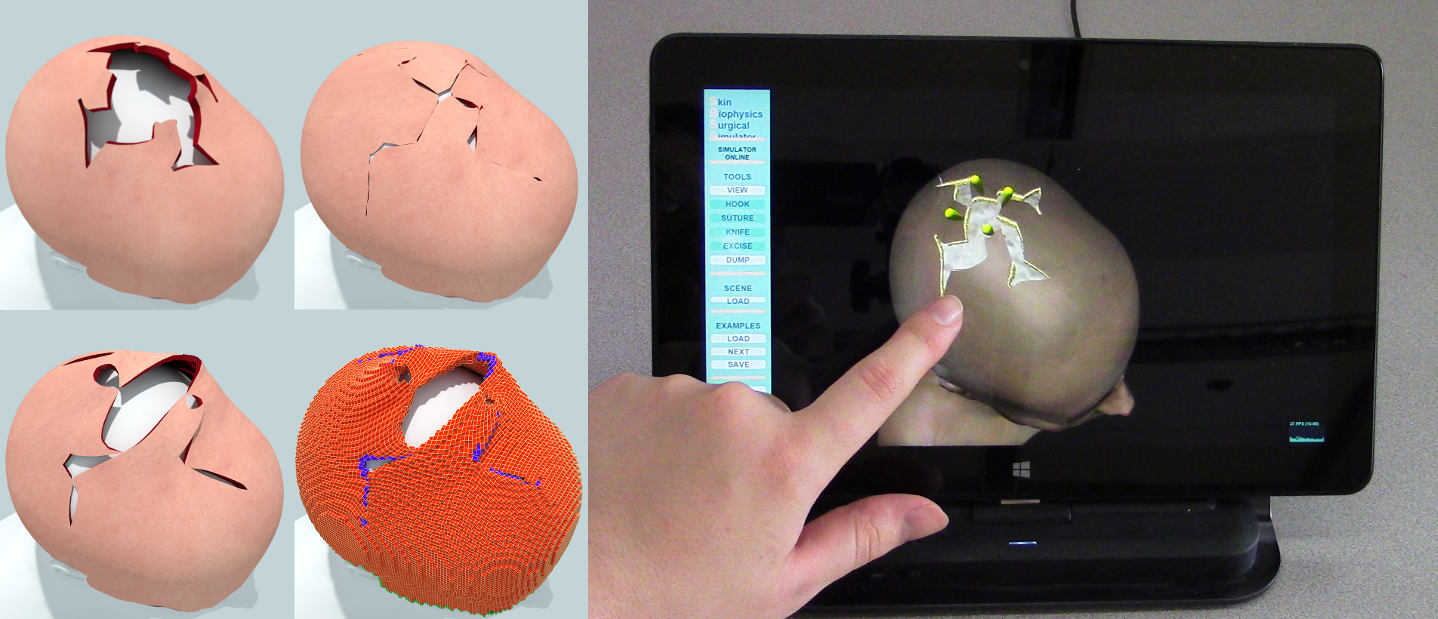
\includegraphics[height=2.99in]{chapter_gridiron/images/TitleImage.png}
  \vspace*{-.05in}
  \caption{Simulation of an advanced surgical repair at the top of the
    scalp}{Simulated \textbf{Dufourmentel-Mouly} repair (see\
    \protect\cite{Baker:2014}) for a large gap of excised tissue on
    the scalp. From top to bottom, left to right: Rendered stages of
    procedure, embedding lattice, real time demo on a tablet running
    in a web browser.}
  \vspace*{-.05in}
  \label{fig:gridiron-teaser}
\end{figure}

\paragraph{Utility} The final \gls{pvis} aspect to discuss in regards
to the plastic surgery domain is that of utility. This topic has been
touched upon in the previous sections on Geometry, Reactivity,
Dynamism, and Interactivity, but here the goal to explore in more
depth how a \gls{pvis} can be used to support the plastic surgery
profession. Surgical skills targeted by computer-based training
solutions have been classified ~\citep{GallaRCHFMSS:2005} in two major
categories. \emph{\Glspl{psymotor}} refer to the dexterous use of
the surgeon's hands to manipulate instruments in the course of an
operation. In plastic surgery, psychomotor training involves
mechanical aspects of surgical tasks, such as the ``feel''
of tissue being cut or the nuances of manipulating a scalpel to enact
a curved incision. For example, training for laparoscopic procedures
requires a clinician to be familiar with the tactile response of
pushing and pulling on organs and to practice coordination
skills required for suturing and cauterization.  A number of
computer-based solutions focus on psychomotor training
~\citep{MendoL:2003,DeKLS:2005,KimCDS:2007,LindbT:2007}.

In contrast to psychomotor training, \emph{cognitive skills} and
training are largely mental rather than dexterous exercises. For
example, in the procedure shown in Figure \ref{fig:gridiron-teaser},
the surgeon needs to contemplate how to best repair a large square
skin defect (i.e. area of excised tissue) by making auxiliary
incisions that create properly shaped ``puzzle pieces'' which can be
sutured together without creating excessive stress. Chentanez et al.\!
\shortcite{ChentARCHGSO:2009} described a cognitive training system
for steerable needle insertion, where the mental challenge lies in
planning a sequence of actions involving needle flexion and torsion,
in order to achieve a desired insertion trajectory.

Focusing on one type of skill training or another affects the design
decisions of a proposed \gls{pvis}. For instance, building a
\gls{pvis} for psychomotor training likely places a greater emphasis
on the interactivity aspects of the system, potentially requiring
haptic feedback mechanisms to provide tactile sensations. Likewise, a
cognitive training aid might require more involved reactivity and
dynamism, such as a more accurate representation of tissue
behaviors. While it might be tempting to say that all aspects, both
psychomotor and cognitive, should be supported equally, it is
important to remember that a \gls{pvis} is not reality. These systems
are fundamentally an approximation of the real world and are subject
to compromises. The next section will explore some of these challenges
in more detail. 

\subsection{PVIS Challenges}

Designing a Practical Visual Interactive System comes with a wide
array of challenges, which is not especially surprising when
considering how many components go into their makeup. In this section,
these challenges will be reviewed, hopefully to give better context
for the design decisions that were made for the rest the work
presented in this document.

\subsubsection{No One Size Fits All?}

During the process of software design, the goal of re-useability is
often discussed. Sometimes designers are referring to reusing
techniques or the software modules, but the theory is more reusable
artifacts are generally more useful. Designing a \gls{pvis}, however,
imposes some interesting roadblocks for the principle of
re-usability. The first issue that often comes up is that the
requirements for a \gls{pvis}, while they can appear similar on the
surface (e.g. display a 3D environment, respond to user input, etc.),
are often implemented with specific optimizations due to the tight
restrictions placed on such systems (e.g. near real-time performance,
extremely complex environments, etc.). Developers faced with these
issues can easily fall into the trap of \textit{blind
  optimization}. This is a form of anti-pattern, where they optimize
the implementation, often quite expertly, for some aspect but without
considering the rest of the system, or later re-usability. It is
important to distinguish this from \textit{premature optimization},
where the developer spends time optimizing an implementation before
knowing if such effort is required. Blind optimization is performed
under local justification. It is only with a broader context that it
can be determined to be a wise course of action. Premature
optimization may end up being wasted effort at best, detrimental at
worst.

Designing general purpose \gls{pvis} platforms is not impossible. Game
developers, over a long developmental history, have created many
excellent general platforms for game development, referred to as game
engines. But increasingly, these platforms, and the developers who
design them, are becoming a field in their own right.  In the past, a
game developer might have done everything from writing low level
graphics code to higher level game logic. In contrast, modern games
are often written by developers who know little about the low level
optimizations required to reach the fidelity and performance expected
by current audiences. Instead, these skills are expressed as game
engines - highly tuned, carefully optimized systems which are not a
game per se, but act as a solid foundation for games written on top of
them. They provide \textit{services}: rendering, resource management,
network support, user interface toolkits, and much more. In essence,
this divide is not dissimilar to that of applications and operating
systems.

The work completed in this document generally follows this
philosophy. As will be described in later sections, the systems
presented in this work adhere to two general principles.

\begin{enumerate}
\item \textbf{Avoid Uncalled for Optimization} During implementation,
  it was important to avoid optimizing too soon. In many cases, there
  were open questions (many still remain!) that premature optimization
  could have prevented a better understanding. Only when it was clear
  that optimization was needed, were further steps taken, and taken in
  complete understanding of their consequences on the rest of the
  system.

\item \textbf{Enforce Clean Separation} As will be discussed in more
  detail in Chapter \ref{chp:deployment}, the domain specific motivation, plastic surgery, was
  separated as much as possible from the underlying enabling
  technologies. This allowed a coupled, but functionally isolated,
  system design, where the components needed to build a plastic
  surgery simulation were isolated from the components needed to build
  a high performance finite element simulator.
  
\end{enumerate}


\subsubsection{Realism and Believability}

For the visual and virtual world aspect of a \gls{pvis}, one primary
question that arises is one of believability or realism. These
concepts are often conflated, though they really should be considered
separately. Realism should be treated as a more direct measure of how
much a user of the system sees what is being presented as an accurate
simulacra of a real object or environment. In contrast, believability
is the measure of how much a user trusts, or is willing to accept, the
information being presented. Lets use modern special effects in
movies, for an example. On one hand, special effects can be used to
introduce elements that have direct real world counterparts, which are
either too expensive or impractical to use. Examples might include
simulating a full ocean, using a green screen to replace environments,
or full simulation of real people. If done well, these techniques
increase realism, by convincing the audience that the elements being
fabricated really exist. On the other hand, special effects can
introduce clearly fantastical elements: mythical creatures, exotic
environments, or magical effects. These are elements that even the
least critical audience member would not hesitate to say are fake. But
the goal here is not to trick them into believing something is real,
but to convince them that its \textit{plausible}. That the fire
breathing dragon, if it were to really exist, would look just like it
does on the screen. This is the believability aspect at work. Of
course, there is no reason that realism and believability can not work
together. Examples include live action heroic characters being
replaced by animated versions in order to have them perform impossible
stunts. Here the result must be have realism (it looks like the real
person), but also be believable (the impossible stunt looks like it
could have been pulled off).

So what does this mean for \gls{pvis} designs in general? And for medical
simulation specifically? The primary issue with a \gls{pvis} is that of user
input. While a movie can be scripted and refined until realism and
believability is exactly where the actors and artists want it to be, a
\gls{pvis} must produce similar levels of fidelity when faced with arbitrary
user actions. Dealing with this challenge often requires domain
specific knowledge in order to limit the potential space of user
interactions. For example, in a surgery simulation, the user can't do
absolutely anything to a section of simulated tissue. They are forced,
by the context of the situation, to interact with it using the
simulated tools provided: scalpels, sutures, etc... This allows a
surgery \gls{pvis} to be engineered to properly handle all the potential
outcomes of this restricted interface, to better produce realistic and
believable results.

\subsubsection{Design Conflicts}

A major problem facing the construction of any \gls{pvis} is that of
design goal conflicts. This is a common software development problem,
where supporting one feature or aspect of a system, such as
performance, comes into direct conflict with implementing another
feature. Continuing with the performance example, suppose we wanted to
impose a strict requirement on visual updates to the user. By doing
so, we have restricted our updates with an upper bound on the maximum
amount of work they can complete at any one time due to time
restrictions. This choice may bias further choices towards the use of
other techniques, not because of any technical merit, but of
complexity.

Many of these conflicting goals exist, some well known in general
software design circles. In the context of physical simulation, there
are several conflicts we need to be especially aware of.


\paragraph{Reactivity Vs. Accuracy}
Before, we touched on general reactivity when discussing the definition
of a \gls{pvis}. For simulation, we can use a more precise definition where the
reactivity of a system refers to the time between a user applies some
change to a simulated system (a force impulse, a constraint change,
etc...) and when the user sees the result of the action. This cause
and effect timing is the reactivity of the system. The smaller this
time, the more reactive the simulation \textit{feels}. We can see this
when comparing the simulation to real materials. For real objects, the
reactivity is effectively infinite, as the time between cause and
effect is extremely close to zero.

Of course, real materials have an advantage that simulated materials
do not. Because they are composed of individual atoms, real objects
effectively act as a perfect finite element simulation, where the
elements are almost infinitely small and operate completely in
parallel to each other. Computer simulated materials are much coarser
in their resolution and, despite great advances in parallel
processing, do not come close to that naturally available in real
materials. Thus, as we increase a simulated object's resolution in
order to capture more and more detail, or use more complex elements
that capture more interesting macroscopic effects, the overall
reactivity of the simulation decreases as more effort is spent
resolving each user action.

The challenge is to find the appropriate balance between the desired
reactivity of a simulation and the accuracy of the simulation. A major
focus of this work has been to explore how both of these aspects can be
increased simultaneously, both by exploiting underutilized parallelism
opportunities and by looking at novel data structures to extract
additional effective resolution without significantly doing so.
  
\paragraph{Domain Utility Vs. Generality}

Another two aspects that often find themselves in conflict for
physical simulation systems are the concepts of domain utility and
generality. Lets look at domain utility first, as it's the more
straightforward of the two. In the simplest terms, domain utility
refers to making design choices in a system that primary serve the
specific task, or domain, that it is currently being built for. This
may refer to choosing or discarding certain features, deciding what
API best suits the current task, or making optimization along critical
paths for the client application. All of these choices can be
reasonable, even correct, as long as you never intend to reuse the
system for any other purpose.

Generality, on the other hand, asks what is the commonality of
different tasks and guides design choices along this route. A general
design should be flexible to different and changing requirements. Such
a system typically eschews APIs built for specific tasks and instead
tries to distill out the fundamental building blocks that any
potential client may need from the system. The difficulties with this
philosophy are two-fold. First, it isn't always obvious what the
fundamental interfaces are, partially because designers by necessity
must look at past applications to define them and are ignorant about
future ones. But secondly, general designs often cannot make
simplifying assumptions that domain specific knowledge provides and
leaves them with overly complex code that tries to optimize for every
use case or simpler code which doesn't optimize anything.

So why would anyone design a general system? On the surface, they seem
harder to build effectively and often don't result in well optimized
solutions, impacting other aspects such as reactivity. The short
answer is flexibility. For a well studied domain, where every last
detail is known and accounted for, a specialized system is probably
the best choice. But in order to answer challenging research
questions, tools and problems often have to change quickly and in
unexpected ways as researchers adapt to new findings and explore new
directions. Medical simulation is very much one of these areas, where
new questions are constantly arising and old preconceptions are
abandoned. As such, during the implementation of the systems described
in this document, considerable effort was spent on creating
generalized simulation systems, and attempting to identify which areas
are ready for optimization and which were not.

 
\subsection{Why Develop a PVIS?}

At this point, a concerned reader may be asking why one should go
through all the trouble of developing these types of systems. The
previous sections have described a complex series of requirements for
\gls{pvis} construction; each one challenging in isolation and more so
in combination. On top of these technical features, there exist higher
level issues, such as problems with generality, user acceptance, and
correctness. Despite all of these problems, developing \gls{pvis}
platforms is doable and ultimately desirable. In order to understand
this position, let us look at the three avenues by which a \gls{pvis}
creates value: As a Catalyst, By Filling a Need, and Intrinsically.

\subsubsection{Catalyst for Advances}

Reasoning about a \gls{pvis} is a complex task, as is the subsequent
process of implementation. In going about this process however, we have
the potential to learn a lot. Anytime we have to adapt a \gls{pvis} to
a new domain or integrate new functionality, we will ultimately
generate questions and hopefully new answers. In this way, \gls{pvis}
implementations are a generator for new research. Whether it is
answering questions about rendering, human-computer interaction,
systems, software design, optimization, or in the case of this thesis,
physical simulation, a \gls{pvis} acts as a fertile soil within which
we, as researchers, are able to experiment in many areas. But more
than simply providing a platform to test isolated ideas, a \gls{pvis}
is by its nature integrated. Any change affects and is affected by
everything else, forcing researchers to take in and understand the big
picture around their work and where it fits into the whole.

\subsubsection{Utility Gap}

The second reason that building a \gls{pvis} is often worthwhile is to
fill a need. A \gls{pvis} is, at its core, software with a purpose. In
some cases, such as game development, many implementations of a
\gls{pvis} have already been created, making the bar much higher as to
the need for another one. But in other areas, such as medical
simulation, the gaps in functionality coverage are more severe. To use
the \gls{pvis} described by this document as an example, there have
been many projects developing systems for laparoscopic organ surgery,
for instance, but few systems for performing simulated plastic
surgery, let alone a fully featured \gls{pvis} with a rich set of
capabilities. Filling this gap with the utility provided by a
\gls{pvis} is then extremely valuable, as without it practitioners are
left behind in a world where their colleagues are more and more
enjoying the benefits of modern computing technology.

\subsubsection{Intrinsic Value}

At a basic level, a \gls{pvis} itself is valuable. Even if we ignore the
value of a \gls{pvis} in fulfilling its specified purpose, or the additional
research that can be spawned as a result of its construction, building
the \gls{pvis} is beneficial to its developers and the greater
community. For the former, implementing a \gls{pvis} requires time,
dedication, and skill - but no one enters and leaves such a project
unchanged. Simply being a developer on a \gls{pvis} helps a developer become
a better software engineer, simply through the long hours of practice
they will spend on it. Beyond individual developers, building a \gls{pvis}
is important to the community at large for the simple reason that it
demonstrates that such a project can be done. Like all large pieces of
software, sometimes the most important idea they can convey is that such a project is
even feasible at all.

%%% Local Variables:
%%% mode: latex
%%% TeX-master: "../document"
%%% End:
